\documentclass[11pt, a4paper, twoside]{article}   	% use "amsart" instead of "article" for AMSLaTeX format

\usepackage{geometry}                		% See geometry.pdf to learn the layout options. There are lots.
\usepackage{pdfpages}
\usepackage{caption}
\usepackage{minted}
\usepackage[german]{babel}			% this end the next are needed for german umlaute
\usepackage[utf8]{inputenc}
\usepackage{color}
\usepackage{graphicx}
\usepackage{titlesec}
\usepackage{fancyhdr}
\usepackage{lastpage}
\usepackage{hyperref}
\usepackage[autostyle=false, style=english]{csquotes}
\usepackage{mathtools}
\usepackage{tabularx}
\usepackage{ulem}
% http://www.artofproblemsolving.com/wiki/index.php/LaTeX:Symbols#Operators
% =============================================
% Layout & Colors
% =============================================
\geometry{
   a4paper,
   total={210mm,297mm},
   left=20mm,
   right=20mm,
   top=20mm,
   bottom=30mm
 }	

\definecolor{myred}{rgb}{0.8,0,0}
\definecolor{mygreen}{rgb}{0,0.6,0}
\definecolor{mygray}{rgb}{0.5,0.5,0.5}
\definecolor{mymauve}{rgb}{0.58,0,0.82}

\setcounter{secnumdepth}{4}


% the default java directory structure and the main packages
\newcommand{\srcDir}{../source/Grammar/}
% =============================================
% Code Settings
% =============================================
\newenvironment{code}{\captionsetup{type=listing}}{}
\newmintedfile[cppSourceFile]{cpp}{
	linenos=true, 
	frame=single, 
	breaklines=true, 
	tabsize=2,
	numbersep=5pt,
	xleftmargin=10pt,
	baselinestretch=1,
	fontsize=\footnotesize
}
\newmintinline[inlineCpp]{cpp}{}
\newminted[cppSource]{cpp}{
	breaklines=true, 
	tabsize=2,
	autogobble=true,
	breakautoindent=false
}

\newcommand{\xvdash}[1]{%
  \vdash^{\mkern-10mu\scriptscriptstyle\rule[-.9ex]{0pt}{0pt}#1}%
}

% =============================================
% Page Style, Footers & Headers, Title
% =============================================
\title{Übung 1}
\author{Thomas Herzog}

\lhead{Übung 1}
\chead{}
\rhead{
\includegraphics[scale=0.10]{FHO_Logo_Students.jpg}}

\lfoot{S1610454013}
\cfoot{}
\rfoot{ \thepage / \pageref{LastPage} }
\renewcommand{\footrulewidth}{0.4pt}
% =============================================
% D O C U M E N T     C O N T E N T
% =============================================
% =============================================
% 2016.10.13: 1 
% 2016.10.14: 2
% =============================================

\pagestyle{fancy}
\begin{document}
\setlength{\headheight}{15mm}
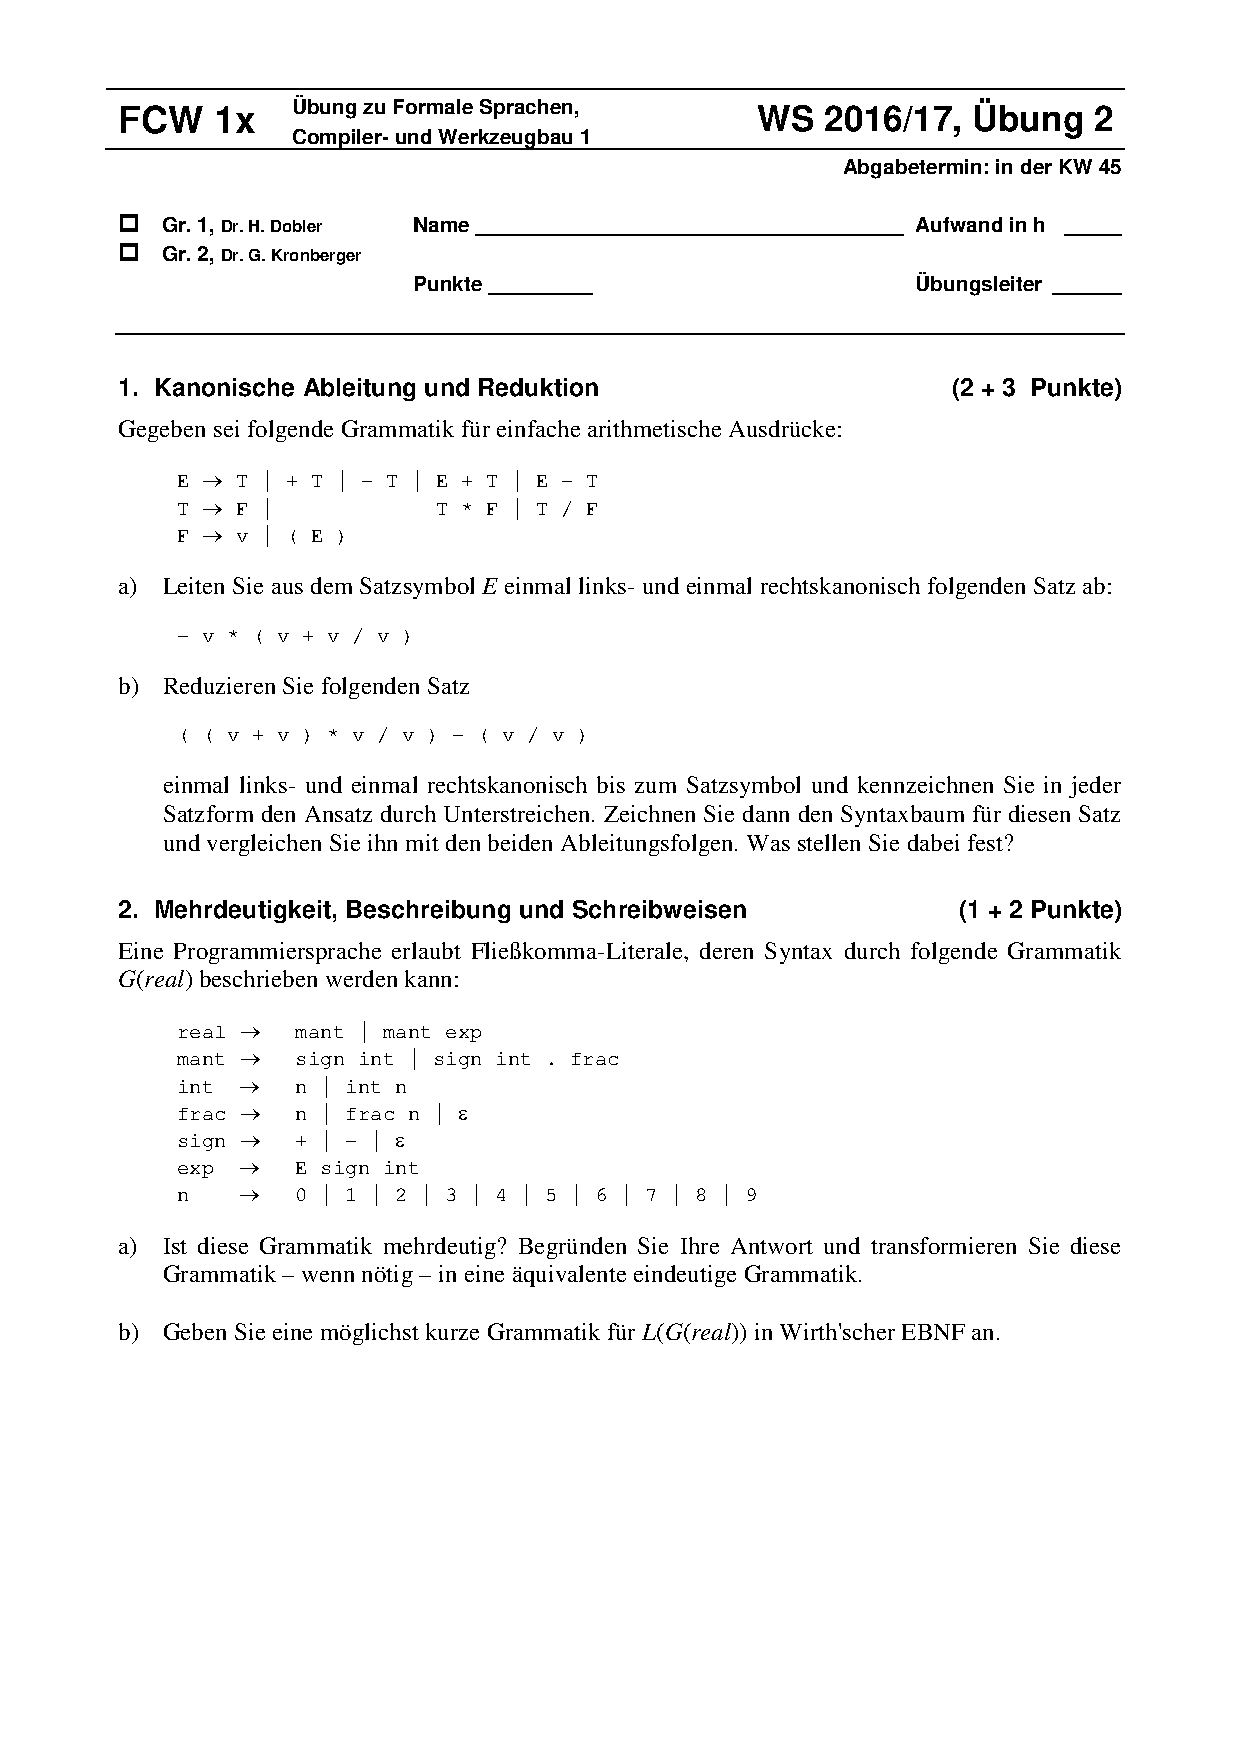
\includepdf[pages={1,2}]{Fcw1x02A.pdf}

% Section gramar and basics 
\section {Kanonische Ableitung und Reduktion}
\label{sec:derive}
Dieser Abschnitt behandelt die Aufgabe 1 der zweiten Übung.
\subsection{Rechtskanonische Ableitung}
Folgende Ableitung beweist, dass der Satz $-v * (v + v / v)$ ein Satz der Sprache ist, die durch die gegebene Grammatik definiert ist.
\newline
\newline
\begin{tabularx}{\textwidth}{p{20pt} @{$\xRightarrow{L}$ \hspace{10pt}} X}
	$E$      & $\underline{-T}$ \\
	         & $\underline{-T} * F$\\
	         & $\underline{-F} * F$\\
	         & $- v * \underline{F}$\\
	         & $- v * (\underline{E})$\\
	         & $- v * (\underline{E} + T)$\\
	         & $- v * (\underline{T} + T)$\\
	         & $- v * (\underline{F} + T)$\\
	         & $- v * (v + \underline{T})$\\
	         & $- v * (v + \underline{T} / F)$\\
	         & $- v * (v + \underline{F} / F)$\\
	         & $- v * (v + v / \underline{F})$\\
	         & $- v * (v + v / v)$\\
\end{tabularx}
\subsection{Kanonische Reduktion}
Folgende Reduktion beweist das der Satz $((v + v) * v / v) - (v / v)$ ein Satz der Sprache ist, die durch die vorgegebene Grammatik definiert ist.
\subsubsection{Linkskanonische Reduktion}
\begin{tabularx}{\textwidth}{p{120pt} @{$\xvdash{L}$ \hspace{10pt}} X}
                  & $((\underline{v} + v) * v / v) - (v / v)$ \\
                  & $((\underline{F} + v) * v / v) - (v / v)$ \\                       
                  & $((\underline{T} + v) * v / v) - (v / v)$ \\                       
                  & $((E + \underline{v}) * v / v) - (v / v)$ \\
                  & $((E + \underline{F}) * v / v) - (v / v)$ \\
                  & $((\underline{E + T}) * v / v) - (v / v)$ \\
                  & $ (\underline{(E}) * v / v) - (v / v)$ \\
                  & $ (\underline{F} * v / v) - (v / v)$ \\
                  & $ (T * \underline{v} / v) - (v / v)$ \\
                  & $ (\underline{T * F} / v) - (v / v)$ \\
                  & $ (T / \underline{v}) - (v / v)$ \\
                  & $ (\underline{T / F}) - (v / v)$ \\
                  & $ (\underline{T}) - (v / v)$ \\
                  & $ (\underline{E}) - (v / v)$ \\
                  & $ \underline{F} - (v / v)$ \\
                  & $ \underline{T} - (v / v)$ \\
                  & $ E - (\underline{v} / v)$ \\
                  & $ E - (\underline{F} / v)$ \\
                  & $ E - (\underline{T} / v)$ \\
                  & $ E - (\underline{T / F})$ \\
                  & $ E - (\underline{T})$ \\
                  & $ E - (\underline{E})$ \\
                  & $ E - \underline{F}$ \\
                  & $ \underline{E - T}$ \\
                  & $ E $ \\
\end{tabularx}

\subsubsection{Rechtskanonische Reduktion}
\begin{tabularx}{\textwidth}{p{120pt} @{$\xvdash{R}$ \hspace{10pt}} X}
                  & $((v + v) * v / v) - (v / \underline{v})$ \\
                  & $((v + v) * v / v) - (\underline{v} / F)$ \\                       
                  & $((v + v) * v / v) - (\underline{F} / F)$ \\                       
                  & $((v + v) * v / v) - (\underline{T / F})$ \\
                  & $((v + v) * v / v) - (\underline{T})$ \\
                  & $((v + v) * v / v) - \underline{(E)}$ \\
                  & $((v + v) * v / v) - \underline{F}$ \\
                  & $((v + v) * v / \underline{v}) - T$ \\
                  & $((v + v) * \underline{v} / F) - T$ \\
                  & $((v + \underline{v}) * F / F) - T$ \\
                  & $((v + \underline{F}) * F / F) - T$ \\
                  & $((\underline{v} + T) * F / F) - T$ \\
                  & $((\underline{F} + T) * F / F) - T$ \\
                  & $((\underline{T} + T) * F / F) - T$ \\
                  & $((\underline{E + T}) * F / F) - T$ \\
                  & $((\underline{E}) * F / F) - T$ \\
                  & $(\underline{F} * F / F) - T$ \\
                  & $(\underline{T * F} / F) - T$ \\
                  & $(\underline{T / F}) - T$ \\
                  & $(\underline{T}) - T$ \\
                  & $(\underline{E}) - T$ \\
                  & $\underline{F} - T$ \\
                  & $\underline{T} - T$ \\
                  & $\underline{E - T}$ \\
                  & $ E $ \\
\end{tabularx}

\section{Mehrdeutigkeit, Beschreibung und Schreibweise}
\subsection{Mehrdeutigkeit der Grammatik}
Folgendes Beispiel zeigt das die vorgegebene Grammatik für den Satz $+ 1.5$ mehrdeutig ist, was durch die Regel $frac \rightarrow \epsilon | fract n $ verursacht wird.
\newline

\begin{figure}[h]
\centering
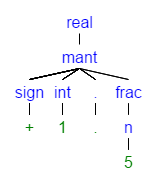
\includegraphics[scale=0.8]{syntax_tree_real_1.png}
\caption{Syntaxbaum 1}
\label{fig:syntaxtree}
\end{figure}
\ \newpage

\begin{figure}[h]
\centering
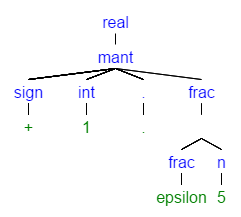
\includegraphics[scale=0.8]{syntax_tree_real_2.png}
\caption{Syntaxbaum 2}
\label{fig:syntaxtree}
\end{figure}
\ \newline


\begin{tabularx}{\textwidth}{p{120pt} @{$\Rightarrow$ \hspace{10pt}} X}
real  & mant $|$ mant exp \\
mant  & sign int $|$ sign int . frac \\
int   & n $|$ int n\\
frac  & n $|$ frac n \\
sign  & + $|$ - \\
exp   & E sign int \\
n     & 0 $|$ 1 $|$ 2 $|$ 3 $|$ 4 $|$ 5 $|$ 6 $|$ 7 $|$ 8 $|$ 9 $|$  $\epsilon$  \\
\end{tabularx}

\subsection{Grammatik mit Wirth'scher Schreibweise}
Folgende Grammatik ist die vorgegebene Grammatik in der Wirth'schen Schreibweise.
\newline
\newline
G = [\enquote{+} $|$ \enquote{+}] n \{n\} [\enquote{.} \{n\} ] [\enquote{E} [\enquote{+} $|$ \enquote{+}] n \{n\}].
\newpage

\section{Reguläre Sprachen}
\subsection{Reguläre Grammatik}
\begin{figure}[h]
\centering
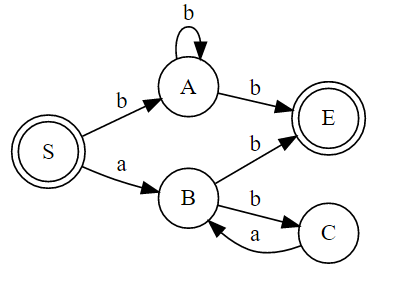
\includegraphics[scale=1]{regular_grammar_automat.PNG}
\caption{Automat}
\label{fig:syntaxtree}
\end{figure}
\ \newline
Folgende Grammatik wurde aus dem Automaten abgeleitet. Diese Grammatik muss aber noch angepasst werden, denn die Regel S $\rightarrow \epsilon$ ist in einer regulären Grammatik nicht gültig.
\newline
\newline
Die folgende Grammatik 
\newline
\begin{tabularx}{\textwidth}{p{20pt} @{$\rightarrow$ \hspace{10pt}} X}
E & Ab $|$ Bb \\                      
A & Ab $|$ \sout{S}b \\
B & \sout{S}a $|$ Ca \\
C & Bb        \\
\sout{S} & \sout{$\epsilon$}\\ 
\end{tabularx}
\ \newline
wird umgeformt zu
\newline
\newline
\begin{tabularx}{\textwidth}{p{20pt} @{$\rightarrow$ \hspace{10pt}} X}
E & Ab $|$ Bb \\                      
A & Ab $|$ b  \\
B & a $|$ Ca  \\
C & Bb        \\ 
\end{tabularx}


\subsection{Umgekehrte reguläre Grammatik}
Die folgende Auflistung zeigt die drei regulären Ausdrücke, welche die Grammatik aus der Aufgabenstellung 3 beschreiben.
\newline
\begin{enumerate}
	\item $\epsilon+$
	\item $bb*b+$
	\item $a(ba)*b$
\end{enumerate}

\subsection{Regulärer Ausdruck der Grammatik}
Folgender regulärer Ausdruck beschreibt die Grammatik aus der Aufgabenstellung 3.
\newline
\newline
$L = \epsilon + bb*b + a(ba)* b$

\section{Bezeichner in der Programmiersprache Ada}
Dieser Abschnitt beschäftigt sich mit der Aufgabenstellung 4 der dritten Übung.

\subsection{Reguälre Grammatik}
\begin{figure}[h]
\centering
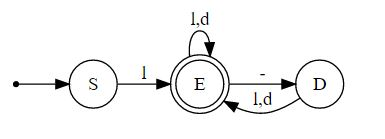
\includegraphics[scale=1]{ada_state_machine.JPG}
\caption{Ada reguläre Grammatik}
\label{fig:ada-state-machine}
\end{figure}

\begin{tabularx}{\textwidth}{p{20pt} @{$\rightarrow$ \hspace{10pt}} X}
S & lE $|$ l \\                      
E & lE $|$ dE $|$ $"\_"$U $|$ l $|$ d \\
U & lE $|$ dE $|$ l $|$ d \\
\end{tabularx}

\subsection{Umgekehrte reguläre Grammatik}
\begin{tabularx}{\textwidth}{p{20pt} @{$\rightarrow$ \hspace{10pt}} X}
E & El $|$ Ed $|$ Ul $|$ Ud $|$ l \\                      
U & E$"\_"$ \\
\end{tabularx}

\subsection{Regulärer Ausdruck}
$l((l+d) + (\_(l+d))*$

\section{Transformation der Darstellungsformen der regulären Sprachen}
\subsection{Reguälre Grammatik}
\begin{figure}[h]
\centering
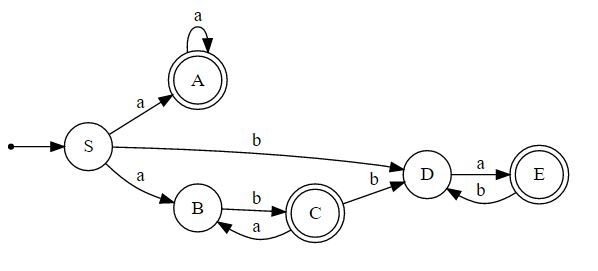
\includegraphics[scale=1]{transformed_regular_exp.JPG}
\caption{Nicht deterministischer Zustandsautomat des transformierten Ausdrucks}
\label{fig:ada-state-machine}
\end{figure}
\ \newline
\textbf{Zustandsüberführungsfunktion}
\newline
\begin{tabularx}{10cm}{p{30pt} XX}
    & a & b \\
 S  & \{A,B\} & \{D\} \\
 A  & \{A\} & \{\} \\
 B  & \{\} & \{C\} \\
 C  & \{B\} & \{D\} \\
 D  & \{E\} & \{\} \\
 E  & \{\} & \{D\} \\
\end{tabularx}
\ \newline
\newline
\newline
\textbf{transformierte Zustandsüberführungsfunktion}
\newline
\begin{tabularx}{10cm}{p{30pt} XX}
    & a & b \\
 S        & \{A,B\} & \{D\} \\
 \{A,B\}  & \{A\} & \{C\} \\
 A        & \{A\} & \{\} \\
 B        & \{\} & \{C\} \\
 C        & \{B\} & \{D\} \\
 D        & \{E\} & \{\} \\
 E        & \{\} & \{D\} \\
\end{tabularx}
\begin{figure}[h]
\centering
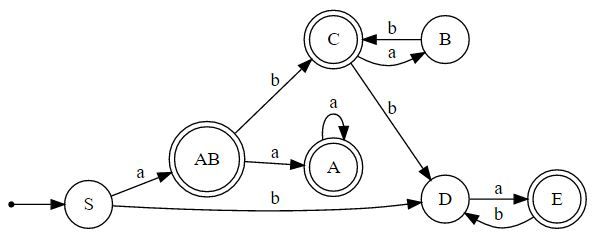
\includegraphics[scale=1]{transformed_regular_exp_determeneistic.JPG}
\caption{Deterministischer Zustandsautomat des transformierten Ausdrucks}
\label{fig:ada-state-machine}
\end{figure}
\end{document}